\documentclass[UTF-8,twoside,cs4size]{ctexart}
\usepackage{amsmath}
\usepackage{amssymb}
\usepackage{geometry}
\usepackage{setspace}
\usepackage{xeCJK}
\usepackage{ulem}
\usepackage{pstricks}
\usepackage{pstricks-add}
\usepackage{bm}
\usepackage{mathtools}
\usepackage{breqn}
\usepackage{mathrsfs}
\usepackage{esint}
\usepackage{textcomp}
\usepackage{upgreek}
\usepackage{pifont}
\usepackage{tikz}
\usepackage{circuitikz}
\usepackage{caption}
\usepackage{xcolor}
\usepackage{tabularx}
\usepackage{array}
\usepackage{pgfplots}
\usepackage{multirow}
\usepackage{pgfplotstable}

\newcolumntype{Y}{>{\centering\arraybackslash}X}
\geometry{a4paper,centering,top=0.75cm,bottom=2.54cm,left=2cm,right=2cm}
\pagestyle{plain}
\captionsetup{font=small}

\CTEXsetup[name={,.}]{section}
\CTEXsetup[format={\raggedright\bfseries\noindent\zihao{3}}]{section}
\CTEXsetup[format={\raggedright\bfseries\quad\large}]{subsection}
\CTEXsetup[format={\raggedright\bfseries\qquad}]{subsubsection}
\renewcommand\thefootnote{\ding{\numexpr171+\value{footnote}}}

\setstretch{1.5}

\setCJKfamilyfont{boldsong}[AutoFakeBold = {2.17}]{SimSun}
\newcommand*{\boldsong}{\CJKfamily{boldsong}}
%\DeclareMathOperator\dif{d\!}
\newcommand*{\me}{\mathop{}\!\mathrm{e}}
\newcommand*{\mpar}{\mathop{}\!\partial}
\newcommand*{\dif}{\mathop{}\!\mathrm{d}}
\newcommand*{\tab}{\indent}

\begin{document}
	\begin{flushright}
		\zihao{2}{分组号:3-07}
	\end{flushright}
	
	\noindent{\zihao{-2}\boldsong\bfseries 《\,\, 基\,\, 础\,\, 物\,\, 理\,\, 实\,\, 验\,\, 》\,\, 实\,\, 验\,\, 报\,\, 告\,\, }
	
	\noindent\textit{实验名称\uline{\quad\qquad\qquad\quad 气轨上弹簧振子的简谐振动\,\qquad\qquad\qquad}指导教师\uline{\qquad\,\,\,赵越\quad\,\,\,\qquad}}
	
	\noindent\textit{姓\qquad 名\uline{\,\,\, 桂庭辉\,\,\,}\,学号\uline{\,\,\,{\upshape2019K8009929019}\,\,\,}\,专\qquad 业\uline{\,\,\,计算机科学与技术\,\,\,}\,班级\uline{\,\,\,\upshape{03}\,\,\,}\,座号\uline{\,\,\,\upshape{6}\,\,\,}}
	
	\noindent\textit{实验日期\uline{\,\,{\upshape 2020}\,\,}年\uline{\,\,{\upshape 12}\,\,}月\uline{\,\,{\upshape02}\,\,}日\,\,实验地点\uline{\,\,\,教学楼{\upshape716}\,\,\,}调课/补课\uline{\,\,\,$ \square $是\,\,\,}成绩评定\uline{\,\,\,\quad\qquad\qquad}}
	
	\begin{table}[h]
		\centering
		\psset{linewidth=2pt}
		\begin{pspicture}(-1,-0.1)(1,0.1)
		\psline(-9,0)(9,0)
		\end{pspicture}
	\end{table}

	\section{实验目的}
	1.观察简谐振动现象,测定简谐振动的周期;
	
	2.求弹簧的倔强系数$ \bar k $和有效质量$ \bar m_0 $;
	
	3.观察简谐振动的运动学特征;
	
	4.验证机械能守恒定律。
	
	\section{实验仪器与用具}
	气垫导轨、滑块、附加砝码、弹簧、U型挡光片、平板挡光片、数字毫秒计、天平等。
	
	{\kaishu 1.气垫导轨是一种近似无阻力的力学试验装置,由气源将压缩空气注入导轨型腔,从导轨表面的小孔喷出气流,在导轨与滑行器之间形成气垫膜,使得滑行器浮起。滑行器在导轨上做近似无阻力的直线运动,使得实验结果近似理论值。}
	
	{\kaishu 2.光电计数器由频率计和光电门两部分构成,频率计相当于时钟,光电门相当于开关。开机后初始化内部参数,启动系统时钟,等待挡光信号。若光电门被遮挡,则相应的光信号被光电接收电路转换成电信号,触发单片机根据系统时钟读取并记录挡光时刻的时间。使用标准挡光距离的挡光片,可以利用计数器计算出速度、加速度等。}
	
	{\kaishu 3.U型挡光片示意图如图1,将其以垂直于导轨的方向安装在滑块上,随滑块在气垫导轨上运动,第一个边$ 11' $刚挡住光时,计时器启动,第三个边$ 33' $挡住光时,计时器再次启动。两边之间的距离为标准值,根据两次挡光的时间即可计算出速度。}
	
	\begin{figure}[!h]
		\centering
		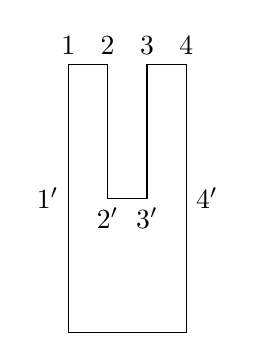
\begin{tikzpicture}
			\draw (0,0)node[left]{$ 1' $}--(0,1.7)node[above]{1}--(0.5,1.7)node[above]{2}--(0.5,0)node[below]{$ 2' $}--(1,0)node[below]{$ 3' $}--(1,1.7)node[above]{3}--(1.5,1.7)node[above]{4}--(1.5,0)node[right]{$ 4' $}--(1.5,-1.7)--(0,-1.7)--(0,0);
		\end{tikzpicture}
		\caption{U型挡光片示意图}
	\end{figure}

	{\kaishu 4.用光电计数器测量条形挡光片第一次挡光和第三次挡光间的时间间隔,便可得到滑块的振动周期。}
	
	\section{实验原理}
	\subsection{弹簧振子的简谐振动}
	如图,在水平气垫导轨上,两个相同的弹簧中间系一滑块,滑块做往返振动。气垫导轨上滑块做近似无阻力的直线运动,则滑块振动可看成简谐振动。
	\begin{figure}[!h]
		\centering
		\begin{circuitikz}
			\draw (-1,-0.5) rectangle (1,0.5);
			\node at(0,0) {滑块};
			\draw (1,0) to[R] (3,0);
			\draw (-1,0) to[R] (-3,0);
			\node[above] at(0,0.5) {$ m_1 $};
			\draw (1,0.6)--(1,1.2);
			\draw (1.8,0.6)--(1.8,1.2);
			\draw [<->] (1.05,0.8)--(1.75,0.8);
			\node[above] at(1.4,0.8) {$ x_0 $};
			\draw (-1,0.6)--(-1,1.2);
			\draw (-1.8,0.6)--(-1.8,1.2);
			\draw [<->] (-1.05,0.8)--(-1.75,0.8);
			\node[above] at(-1.4,0.8) {$ x_0 $};
			\node[below] at(-2,0) {$ k_1 $};
			\node[below] at(2,0) {$ k_1 $};
			\draw (0,-1)--(3,-1)--(3,0.6)--(3.3,0.6)--(3.3,-2)--(-3.3,-2)--(-3.3,0.6)--(-3,0.6)--(-3,-1)--(0,-1);
			\node at(0,-1.5) {气垫导轨};
		\end{circuitikz}
		\caption{简谐运动原理图}
	\end{figure}
	
	设滑块(与其上重物)的总质量为$ m_1 $,其位于平衡位置,每个弹簧的伸长量均为$ x_0 $。当$ m_1 $距平衡点$ x $时,其只受来自两个弹簧的弹性力作用\footnote{水平方向上。竖直方向上,受力平衡不参与牛顿第二定律方程的导出。},记弹簧的倔强系数为$ k_1 $,根据牛顿第二定律可知运动方程为
	\[-kx=ma\]
	其中$ k=2k_1,\;m=m_0+m_1 $,$ m $为振动系统的有效质量,$ m_0 $为弹簧的有效质量,$ a $为滑块加速度。求解该方程有
	\begin{equation}\label{3-1-1}
		x=A\sin(\omega_0t+\varphi_0)	
	\end{equation}
	其中$ A $为振幅,$ \varphi_0 $为初相位,$ \omega_0=\sqrt{\frac km} $为振动系统的固有频率,由振动系统本身的性质所决定。
	
	可求得振动周期$ T $为
	\[T=\frac{2\pi}{\omega_0}=2\pi\sqrt{\frac mk}=2\pi\sqrt{\frac{m_0+m_1}{k}}\]
	上式两边平方即得
	\begin{equation}\label{3-1-2}
		T^2=4\pi^2\frac{m_0+m_1}{k}	
	\end{equation}
	
	\subsection{简谐运动的运动学特征描述}
	对式(\ref{3-1-1})在时间上求导得:
	\begin{equation}\label{3-2-1}
		v=\frac{\dif x}{\dif t}=A\omega_0\cos(\omega_0t+\varphi_0)
	\end{equation}
	由上式可知速度$ v $随时间变化做简谐振动,角频率为$ \omega_0 $,振幅为$ A\omega_0 $,其相位比$ x $超前$ \frac\pi2 $.
	
	由式(\ref{3-1-1}),(\ref{3-2-1}),消去时间$ t $可得
	\[v^2=\omega_0^2(A^2-x^2)\]
	
	\subsection{简谐振动的机械能}
	在本次实验中任意时刻,系统的振动动能为
	\[E_k=\frac12mv^2=\frac12(m_0+m_1)v^2\]
	弹性势能\footnote{记$ m_1 $位于平衡位置时系统的弹性势能为零。}为
	\[E_p=\frac12kx^2\]
	系统的机械能
	\begin{equation}\label{3-3-3}
		E=E_k+E_p=\frac12m\omega^2A^2=\frac12kA^2
	\end{equation}
	其中$ k,A $不随时间发生变化。通过测量滑块在不同位置$ x $的速度$ v $,从而计算弹性势能和振动势能,并可验证他们之间的相互转换关系与机械能守恒定律。
	
	\section{实验内容}
	1.学习使用光电计数器测量速度、加速度、周期的方法。
	
	2.调节气垫导轨至水平,通过测量任意两点间的速度变化,对气垫导轨进行调平。
	
	3.测量弹簧振子的振动周期并考察振动周期与振幅的关系。分别取滑块振幅$ A $为10.0,\ 20.0,\ 30.0,\ 40.0\,cm时,测量其相应振动周期。分析和讨论实验结果。
	
	4.探究振动周期与振子质量之间的关系。在滑块上加骑码(铁片)。对一个确定的振幅,每增加一个骑码\footnote{但骑码不能加太多,需保证阻尼不明显。}测量一组$ T $。作出$ T^2-m $图象,根据公式(\ref{3-1-2})可知图象应为一直线,其斜率为$ \frac{4\pi^2}{k} $,截矩为$ \frac{4\pi^2m_0}{k} $,用最小二乘法作出拟合直线即可求得$ k,m_0 $.
	
	5.研究速度与位移间的关系,在滑块上加装U型挡光片,可测量速度。作出$ v^2-x^2 $图象,做拟合直线,验证斜率是否为$ -\omega_0^2 $,截距是否为$ A^2\omega_0^2 $,其中$ \omega_0=\frac{2\pi}{T} $,其中$ T $可测出。
	
	6.探究振动系统的机械能是否守恒。固定振幅,在不同$ x $处测出滑块速度,由此计算出振动过程中每经过一个$ x $处的动能和势能,并对各$ x $处的机械能进行比较,验证机械能守恒。
	
	7.根据式(\ref{3-3-3}),改变振幅$ A $,测得相应的$ v_{\max} $,由$ v_{\max}^2-A^2 $图象求$ k $,与第4步结果进行比较。
		
	\section{实验结果与数据处理}
	\subsection{实验仪器的调试}
	通过粗调使得滑块在气垫导轨上没有明显移动或在较小范围内做往复运动。安装两个光电门,在滑块上安装测量速度的U型挡光片,测得分别通过两个光电门的速度,相应调节高度直至通过两光电门的速度相差不大。最终测得数据如下:
	
	\begin{table}[!h]
		\centering
		\renewcommand\arraystretch{1.5}
		\begin{tabularx}{\textwidth}{|Y|Y|Y|}
			\hline
			$ v_1 $\;(cm/s)&$ v_2 $\;(cm/s)&误差\;\%\\
			\hline
			103.30&102.88&0.407\\
			\hline
			95.97&95.69&0.292\\
			\hline
			99.50&99.11&0.392\\
			\hline
		\end{tabularx}
		\caption{调平气垫导轨数据记录}
	\end{table}

	上表中每行误差均在0.5\%内,可认为导轨已调平。
	
	\subsection{测量弹簧振子的振动周期并考察振动周期和振幅的关系}\label{A-T}
	滑块振幅$ A $分别为10.0,\;20.0,\;30.0,\;40.0\,cm时,测量相应振动周期,每组数据测量五个周期取平均值:
	\begin{table}[!h]
		\centering
		\renewcommand\arraystretch{1.5}
		\begin{tabularx}{\textwidth}{|c|Y|Y|Y|Y|}
			\hline
			$ A $\;(cm)&10&20&30&40\\
			\hline
			$ T_1 $\;(ms)&1578.69&1577.89&1577.53&1577.63\\
			\hline
			$ T_2 $\;(ms)&1577.91&1578.23&1577.80&1577.80\\
			\hline
			$ T_3 $\;(ms)&1578.25&1577.60&1577.87&1578.17\\
			\hline
			$ T_4 $\;(ms)&1578.88&1577.58&1577.48&1578.17\\
			\hline
			$ T_5 $\;(ms)&1578.77&1577.84&1577.92&1578.02\\
			\hline
			$ T $\;(ms)&1578.50&1577.83&1577.72&1577.96\\
			\hline
		\end{tabularx}
		\caption{不同振幅下弹簧振子的振动周期}
	\end{table}

	在误差允许的范围内,可以认为最终结果中的四个周期相同,即振动周期与振幅无关。这一点在实验原理部分也可得到验证:振动周期$ T $仅与振动系统自身性质(振动系统的有效质量、弹簧的倔强系数)有关,而与振幅等无关。
	
	\subsection{研究振动周期与振子质量之间的关系}\label{km}
	实验测得滑块质量为219.48\,g,测周期时所用条形挡光片质量为1.89\,g,依次加上四个质量在12.5\,g左右的骑码,测量相应的振动周期,测量结果如下表:
	\begin{table}[!h]
		\centering		
		\renewcommand\arraystretch{1.5}
		\begin{tabularx}{\textwidth}{|c|Y|Y|Y|Y|Y|}
			\hline
			骑码质量$ m $\;(g)&0&12.49&25.03&37.41&49.88\\
			\hline
			振子质量$ M $\;(g)&221.37&233.86&246.40&258.78&271.25\\
			\hline
			$ T_1 $\;(ms)&1577.99&1621.04&1662.79&1703.82&1743.65\\
			\hline
			$ T_2 $\;(ms)&1577.85&1620.62&1662.56&1703.73&1743.71\\
			\hline
			$ T_3 $\;(ms)&1577.79&1620.93&1662.87&1703.52&1743.98\\
			\hline
			$ T_4 $\;(ms)&1578.02&1621.06&1662.68&1703.66&1744.02\\
			\hline
			$ T_5 $\;(ms)&1577.94&1621.02&1662.54&1703.53&1744.10\\
			\hline
			$ T_6 $\;(ms)&1577.82&1621.16&1663.03&1703.49&1743.94\\
			\hline
			$ T_7 $\;(ms)&1577.65&1620.91&1662.90&1703.98&1743.70\\
			\hline
			$ T_8 $\;(ms)&1577.99&1620.94&1662.99&1703.43&1744.04\\
			\hline
			$ T_9 $\;(ms)&1578.11&1620.80&1662.66&1703.63&1744.09\\
			\hline
			$ T_{10} $\;(ms)&1577.81&1621.22&1662.97&1703.45&1744.23\\
			\hline
			$ T $\;(ms)&1577.90&1620.97&1662.80&1703.62&1743.95\\
			\hline
			$ T^2 $\;(s$ ^2 $)&2.4897&2.6275&2.7649&2.9023&3.0413\\
			\hline
		\end{tabularx}
		\caption{不同质量振子的振动周期}
	\end{table}

	根据最小二乘法可求得:
	\(k=\frac{4\pi^2}{11.05}\,\mathrm{N/m}=3.5727\,\mathrm{N/m},\quad m_0=\frac{4.24\times10^{-2}}{11.05}\,\mathrm{kg}=3.8371\,\mathrm{g}\)。
	作出图象如下
	\begin{figure}[!h]
		\centering
		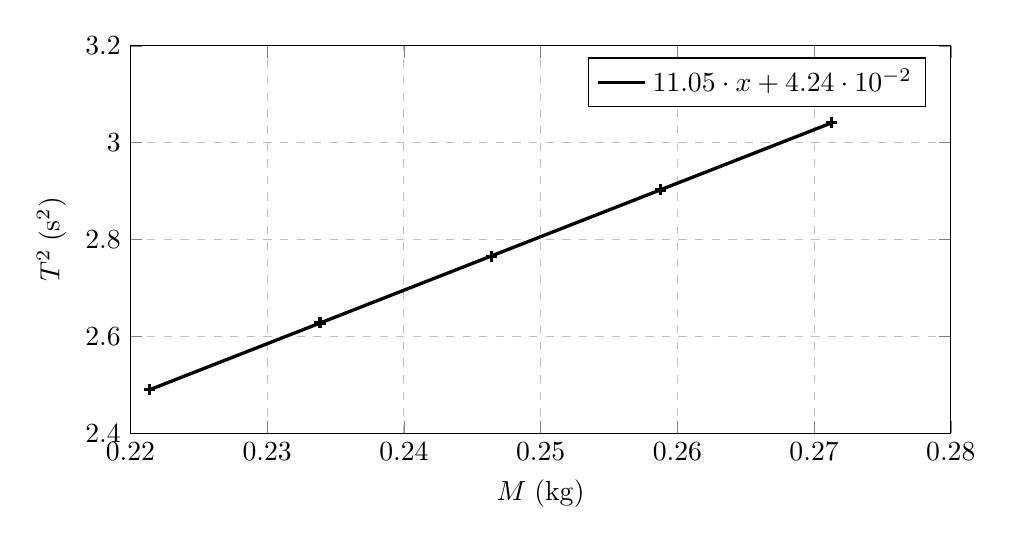
\begin{tikzpicture}
			\begin{axis}[
				legend pos=north east,
				width=12cm,height=6.5cm,
				xlabel=$ M\;(\mathrm{kg}) $,
				ylabel=$ T^2\;(\mathrm{s^2}) $,
				xmin=0.220,xmax=0.280,
				ymin=2.4,ymax=3.2,
				xtick={0.220,0.23,0.240,0.25,0.260,0.27,0.280},
				ytick={2.4,2.6,2.8,3.0,3.2},
				grid style=dashed,
				ymajorgrids=true,
				xmajorgrids=true,
				]
				\addplot[no marks,black,very thick] table[y={create col/linear regression={y=Y}}]
				{
					X	Y
					0.22137	2.4897
					0.23386	2.6275
					0.24640	2.7649
					0.25878	2.9023
					0.27125	3.0413			
				};
				\addlegendentry{
					$\pgfmathprintnumber{\pgfplotstableregressiona} \cdot x
					\pgfmathprintnumber[print sign]{\pgfplotstableregressionb}$}
				
				\addplot [very thick,mark=+,only marks] coordinates {
					(0.22137,2.4897)(0.23386,2.6275)(0.24640,2.7649)(0.25878,2.9023)
					(0.27125,3.0413)
				};
			\end{axis}
		\end{tikzpicture}
		\captionsetup{skip=0pt}
		\caption{$ T^2-M $拟合图象}
	\end{figure}

	由于$ k=k_1+k_2 $,而实验中所用两弹簧可视作相同,即$ k_1=k_2=\frac k2=1.7864\,\mathrm{N/m} $
	
	\subsection{探究速度和位移的关系}
	取固定振幅,分别测量五个不同位置振子的速度,每个位置取三次测量数据的平均值,数据记录如下:
	\begin{table}[!h]
		\centering		
		\renewcommand\arraystretch{1.5}
		\begin{tabularx}{\textwidth}{|c|Y|Y|Y|Y|Y|}
			\hline
			$ x $\;(cm)&10&15&20&25&30\\
			\hline
			$ x^2 $\;(m$ ^2 $)&0.01&0.0225&0.04&0.0625&0.09\\
			\hline
			$ v_1\;(\mathrm{cm/s}) $&151.98&145.77&135.50&123.30&102.25\\
			\hline
			$ v_2\;(\mathrm{cm/s}) $&151.74&145.14&135.57&122.92&102.56\\
			\hline
			$ v_3\;(\mathrm{cm/s}) $&151.52&145.98&135.14&123.61&102.67\\
			\hline
			$ \bar v\;(\mathrm{cm/s}) $&151.75&145.63&135.40&123.28&102.49\\
			\hline
			$ v^2\;(\mathrm{m^2/s^2}) $&2.3028&2.1208&1.8333&1.5198&1.0504\\
			\hline
		\end{tabularx}
		\caption{不同位置的振子速度}
	\end{table}
	
	根据上表可作出如下$ v^2-x^2 $图象:
	
	\begin{figure}[!h]
		\centering
		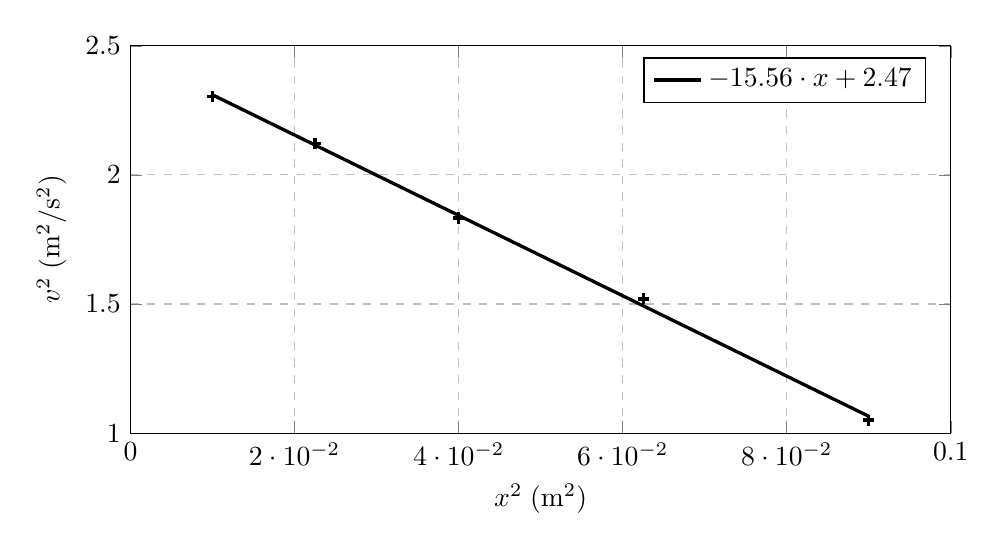
\begin{tikzpicture}
			\begin{axis}[
				legend pos=north east,
				width=12cm,height=6.5cm,
				xlabel=$ x^2\;(\mathrm{m^2}) $,
				ylabel=$ v^2\;(\mathrm{m^2/s^2}) $,
				xmin=0,xmax=0.10,
				ymin=1,ymax=2.5,
				xtick={0,0.02,0.04,0.06,0.08,0.10},
				ytick={1,1.5,2,2.5},
				grid style=dashed,
				ymajorgrids=true,
				xmajorgrids=true,
				]
				\addplot[no marks,black,very thick] table[y={create col/linear regression={y=Y}}]
				{
					X	Y
					0.01	2.3028
					0.0225	2.1208
					0.04	1.833
					0.0625	1.5198
					0.09	1.0504			
				};
				\addlegendentry{
					$\pgfmathprintnumber{\pgfplotstableregressiona} \cdot x
					\pgfmathprintnumber[print sign]{\pgfplotstableregressionb}$}
				
				\addplot [very thick,mark=+,only marks] coordinates {
					(0.01,2.3028)(0.0225,2.1208)(0.04,1.833)(0.0625,1.5198)
					(0.09,1.0504)
				};
			\end{axis}
		\end{tikzpicture}		
	\end{figure}

	由图中点$ (x^2,v^2) $均匀分布在拟合直线附近可知$ v^2 $与$ x^2 $间有负相关的线性关系。根据实验原理$ v^2=\omega_0^2(A^2-x^2) $可知拟合直线斜率即为$ -\omega_0^2 $,截距为$ A^2\omega_0^2 $。
	
	复用\ref{A-T}节中$ A=40.0\,\mathrm{cm}=0.4\,\mathrm{m} $时的振动周期$ T=1577.96\,\mathrm{ms}=1.57796\,\mathrm{s} $,可求得
	\[-\omega_0^2=-\frac{4\pi^2}{T^2}=-15.86\,\mathrm{s^{-2}},\quad A^2\omega_0^2=2.54\,\mathrm{m^2/s^2}\]
	计算结果与本节所做拟合直线的斜率、截距均分别近似相等,可验证$ v^2=\omega_0^2(A^2-x^2) $关系。
	\newpage
	
	\subsection{研究振动系统的机械能是否守恒}
	固定振幅,测出不同位置的滑块速度(复用上节数据),由此可计算得到振动过程中这些位置的动能与势能。测量速度所用U型挡光片质量测得为3.66\,g。复用此前测得的弹簧有效质量$ m_0=3.8371\,\mathrm g $,倔强系数$ k=3.5727\,\mathrm{N/m} $。数据记录如下
	\begin{table}[!h]
		\centering
		\renewcommand\arraystretch{1.5}
		\begin{tabularx}{\textwidth}{|c|Y|Y|Y|Y|Y|}			
			\hline
			$ x $\;(cm)&10&15&20&25&30\\
			\hline
			$ x^2 $\;(m$ ^2 $)&0.01&0.0225&0.04&0.0625&0.09\\
			\hline
			$ v\;(\mathrm{cm/s}) $&151.75&145.63&135.40&123.28&102.49\\
			\hline
			$ v^2\;(\mathrm{m^2/s^2}) $&2.3028&2.1208&1.8333&1.5198&1.0504\\
			\hline
			$ E_k=\frac12(m_0+m_1)v^2\;(\mathrm J) $&0.2613&0.2407&0.2081&0.1725&0.1192\\
			\hline
			$ E_p=\frac12kx^2\;(\mathrm J) $&0.0178&0.0402&0.0715&0.1116&0.1608\\
			\hline
			$ E=E_k+E_p\;(\mathrm J) $&0.2791&0.2809&0.2796&0.2841&0.2800\\
			\hline
		\end{tabularx}
		\caption{验证机械能守恒数据记录}
	\end{table}

	理论上\footnote{指根据测得的倔强系数与原理公式$ E=\frac12kA^2 $}可计算得到系统总机械能
	\[E=\frac 12kA^2=0.2858\,\mathrm J\]
	根据上表数据可作出如下图象
	\begin{figure}[!h]
		\centering
		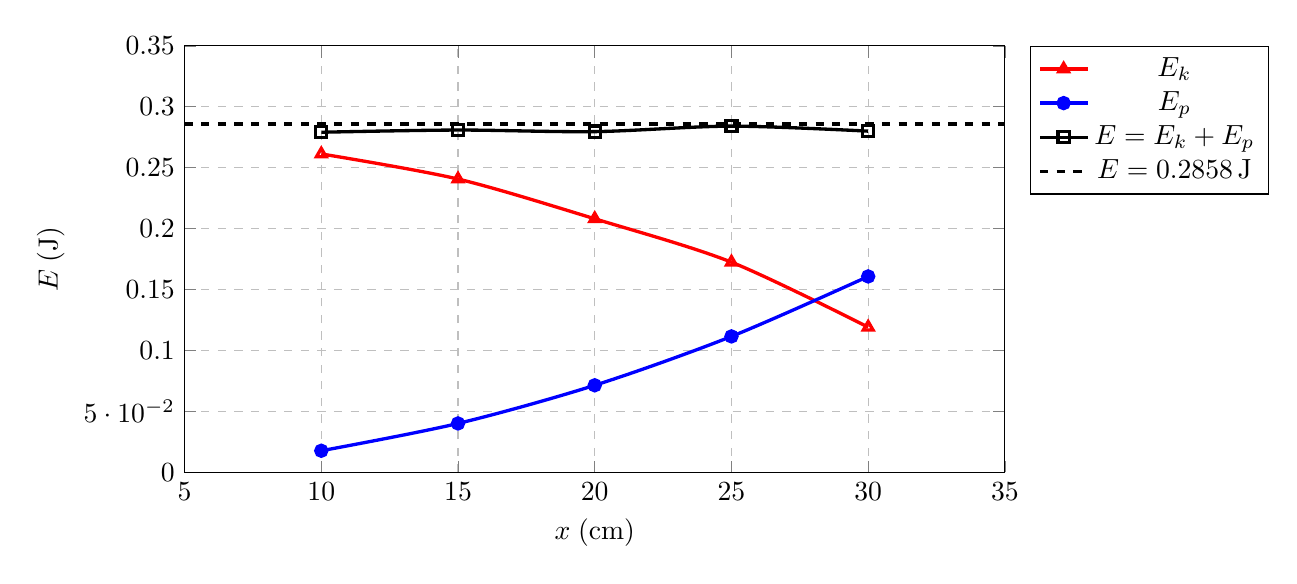
\begin{tikzpicture}
			\begin{axis}[
				legend pos=outer north east,
				width=12cm,height=7cm,
				xlabel=$ x\;(\mathrm{cm}) $,
				ylabel=$ E\;(\mathrm{J}) $,
				xmin=5,xmax=35,
				ymin=0,ymax=0.35,
				xtick={5,10,15,20,25,30,35},
				ytick={0,0.05,0.1,0.15,0.2,0.25,0.3,0.35},
				grid style=dashed,
				ymajorgrids=true,
				xmajorgrids=true,
				]
%				\addplot[no marks,black,very thick] table[y={create col/linear regression={y=Y}}]
%				{
%					X	Y
%					0.01	2.3028
%					0.0225	2.1208
%					0.04	1.833
%					0.0625	1.5198
%					0.09	1.0504			
%				};
%				\addlegendentry{
%					$\pgfmathprintnumber{\pgfplotstableregressiona} \cdot x
%					\pgfmathprintnumber[print sign]{\pgfplotstableregressionb}$}
				
				\addplot [very thick,red,mark=triangle,smooth] coordinates {
					(10,0.2613)(15,0.2407)
					(20,0.2081)
					(25,0.1725)(30,0.1192)
				};
				\addlegendentry{$ E_k $}
				
				\addplot [very thick,blue,mark=*,smooth] coordinates {
					(10,0.0178)(15,0.0402)
					(20,0.0715)
					(25,0.1116)(30,0.1608)
				};
				\addlegendentry{$ E_p $}
				
				\addplot [very thick,mark=square,smooth] coordinates {
					(10,0.2791)(15,0.2809)
					(20,0.2796)
					(25,0.2841)(30,0.2800)
				};
				\addlegendentry{$ E=E_k+E_p $}
				
				\addplot [very thick,dashed,domain=5:35] {0.2858+0*x};
				\addlegendentry{$ E=0.2858\,\mathrm J $}
			\end{axis}
		\end{tikzpicture}
		\caption{$ E_k,\,E_p,\,E_k+E_p $与位移$ x $的关系}
	\end{figure}

	由上图可知,在误差允许的范围内,可认为振动系统的机械能保持恒定,且与计算值近似相等。
	
	\newpage
	\subsection{根据$ v_\max^2-A^2 $关系求$ k $}
	实验数据记录如下:
	\begin{table}[!h]
		\centering		
		\renewcommand\arraystretch{1.5}
		\begin{tabularx}{\textwidth}{|c|Y|Y|Y|Y|Y|}
			\hline
			$ A $\;(cm)&10&15&20&25&30\\
			\hline
			$ A^2 $\;(m$ ^2 $)&0.01&0.0225&0.04&0.0625&0.09\\
			\hline
			$ v_{\max 1} $\;(cm/s)&39.20&57.54&78.49&98.52&118.06\\
			\hline
			$ v_{\max 2} $\;(cm/s)&39.70&57.37&78.99&98.42&118.76\\
			\hline
			$ v_{\max 3} $\;(cm/s)&39.57&57.84&78.68&98.23&118.48\\
			\hline
			$ \bar v_{\max} $\;(cm/s)&39.49&57.58&78.72&98.39&118.43\\
			\hline
			$ v^2_{\max} $\;(m$ ^2 $/s$ ^2 $)&0.1559&0.3315&0.6197&0.9681&1.4026\\
			\hline
		\end{tabularx}
		\caption{不同振幅下振子最大速度}
	\end{table}
	
	根据上表数据可作出如下拟合曲线:
	\begin{figure}[!h]
		\centering
		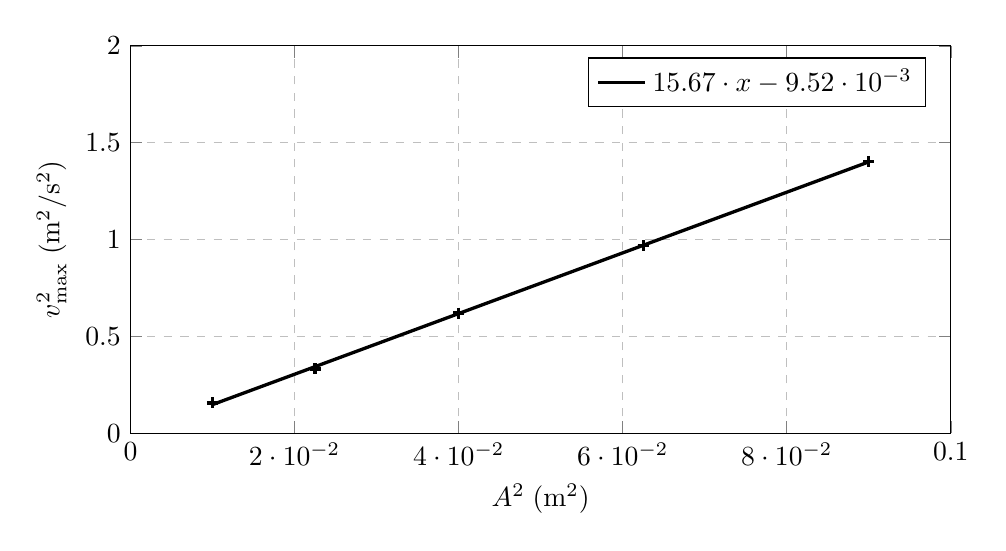
\begin{tikzpicture}
			\begin{axis}[
				legend pos=north east,
				width=12cm,height=6.5cm,
				xlabel=$ A^2\;(\mathrm{m^2}) $,
				ylabel=$ v_\max^2\;(\mathrm{m^2/s^2}) $,
				xmin=0,xmax=0.10,
				ymin=0,ymax=2,
				xtick={0,0.02,0.04,0.06,0.08,0.10},
				ytick={0,0.5,1,1.5,2},
				grid style=dashed,
				ymajorgrids=true,
				xmajorgrids=true,
				]
				\addplot[no marks,black,very thick] table[y={create col/linear regression={y=Y}}]
				{
					X	Y
					0.01	0.1559
					0.0225	0.3315
					0.04	0.6197
					0.0625	0.9681
					0.09	1.4026			
				};
				\addlegendentry{
					$\pgfmathprintnumber{\pgfplotstableregressiona} \cdot x
					\pgfmathprintnumber[print sign]{\pgfplotstableregressionb}$}
				
				\addplot [very thick,mark=+,only marks] coordinates {
					(0.01,0.1559)(0.0225,0.3315)(0.04,0.6197)(0.0625,0.9681)
					(0.09,1.4026)
				};
			\end{axis}
		\end{tikzpicture}		
	\end{figure}

	图象斜率为\[ \omega_0^2=\frac km=15.67\,\mathrm{s^{-2}}\;\Longrightarrow\; k=3.5567\,\mathrm{N/m}\]
	与\ref{km}节中测得的$ k=3.5727\,\mathrm{N/m} $近似相等。
	\section{实验总结}
	\subsection{思考题}
	1.仔细观察,可以发现滑块的振幅是不断减小的,那么为什么还可以认为滑块是做简谐振动?实验中应如何尽量保证滑块做简谐振动?
	
	{\kaishu 气垫导轨虽能显著减小滑块与导轨间的滑动摩擦,但不能将其完全消除,同时也不能排除空气阻力等其他阻力,故而滑块振幅会不断减小,但这部分摩擦力很小,在误差允许的范围内可以忽略。同时,实验实际操作中也会考虑到阻尼对实验结果的影响,故而选择了多次测量取平均、仅保留第一个数据等方式来进一步消除阻尼的影响,从而可认为滑块是做简谐振动的。}
	
	{\kaishu 为保证滑块做简谐振动,实验中可以通过尽可能精调气垫导轨至水平,具体表现为在调平过程中在较小的速度$ v_1,\,v_2 $下仍能保证二者误差不超过0.5\%.}
	
	~\
	
	2.试说明弹簧的等效质量的物理意义,如不考虑弹簧的等效质量,则对实验结果有什么影响?
	
	{\kaishu 在理论模型或推导中,通常认为弹簧是轻质的,但在实验中弹簧具有一定质量,故而会获得一部分动能。弹簧的等效质量即为弹簧的等效质量的物理意义是参与滑块的运动的需要计算动能的一部分质量,也可看作等效给滑块增加的质量。其具体大小推导\footnote{此处推导过程参考自:《振动力学》,刘延柱等,高等教育出版社,1998年版,第9页,例1.1-1}如下:}
		
	{\kaishu 设弹簧长度为$ l $,线密度为$ \rho_l $,弹簧的形变与距固定点距离$ \xi $成正比,弹簧端点的位移为$ x $。取长度为$ \dif\xi $的微元,将其动能在整个弹簧长度上积分,计算弹簧的动能$ E $,得到:}	
	\[E_1=\frac12\rho_l\int_0^l\left(\frac{\dot x\xi}{l}\right)^2\dif\xi=\frac12\left(\frac{m_1}{3}\right)\dot x^2\]
	{\kaishu 其中$ m_1=\rho_ll $为弹簧质量,称式中$ \frac{m_1}{3} $为弹簧的等效质量$ m_e $,记振子的质量为$ m $,则考虑弹簧质量的系统总动能为}
	\[E=\frac12(m+m_e)\dot x^2\]
	
	{\kaishu 实验中若不考虑弹簧的等效质量,则计算出的动能偏小,可能导致无法验证机械能守恒或在利用$ v_\max^2-x^2 $关系计算$ k $的时候结果偏小。}
	
	~\
	
	3.测量周期时,光电门是否必须在平衡位置上?如不在平衡位置会产生什么不同的结果?
	
	{\kaishu 理论上测量周期时不需要把光电门放置在平衡位置上,因为在振幅范围内任意位置固定后,光电门取相邻两个周期内该处对应的同相位点,其之间的时间差均为一个周期。但实际实验过程中,由于无法完全消除阻尼,简谐振动的振幅会不断缩小,那么非平衡点位置在不同周期内对应的相位点将会不同,将会造成振动周期的测量误差甚至挡光片无法完成挡光。所以实际实验中需要将光电门固定在平衡位置上。}
	
	~\
	
	4.气垫导轨如果不水平,是否能进行该实验?
	
	{\kaishu 理论上即便气垫导轨不水平,弹簧仍可做简谐振动,考虑导轨倾斜的角度将重力考虑进来即可进行实验。但实际实验中这样会带来许多数据处理上的麻烦,导轨倾斜角度也可能过小而难以测量,所以应尽可能将气垫导轨调整为水平状态。}
	
	\subsection{心得体会与反思}
	由于数字毫秒计已经完成了一部分的数据处理工作,本次实验的大部分步骤与数据处理工作都得到了简化,主要的精力与时间放在了导轨的调平工作上。我一开始选取的滑块测试速度都较小,仅有20$ \sim $30\,cm/s,要保证误差在0.5\%之内则对导轨调平的精度提出了很高的要求,但实际后续实验对导轨调平的精度要求并没有这么高。如规定振幅$ A=40\,\mathrm{cm} $的几个实验中滑块在平衡位置的速度都超过了$ 100\,\mathrm{cm/s} $,故而可在调平过程中适当放宽测试速度与调平精度,从而节省时间,避免不必要的精力浪费。
\end{document}